Considera la funció
\[
f(x)=\frac{x^2}{x-1} .
\]

\begin{apartats}

\apartat[1,25]{1}
Troba'n el domini, els punts de tall amb els eixos i totes les asímptotes.

\begin{solucio}
\textbf{Domini}: $\mathbb{R}\setminus\{1\}$.\\
\textbf{Talls}: $f(x)=0$ només si $x^2=0$, i $f(0)=0$: la gràfica passa per l'origen
$(0,0)$, que és alhora el tall amb els dos eixos.\\
\textbf{Vertical}: en $x=1$ el numerador val $1\neq0$, i els laterals valen $-\infty$ (per
l'esquerra) i $+\infty$ (per la dreta): asímptota $\boxed{x=1}$.\\
\textbf{Obliqua}: dividint, $\dfrac{x^2}{x-1}=x+1+\dfrac{1}{x-1}$, i el residu tendeix a $0$:
asímptota $\boxed{y=x+1}$. No hi ha asímptota horitzontal.
\end{solucio}

\begin{nomesllarg}
\apartat{0,75}
Estudia'n la curvatura.

\begin{solucio}
$f'(x)=\dfrac{x^2-2x}{(x-1)^2}$ i, derivant un altre cop i simplificant,
$f''(x)=\dfrac{2}{(x-1)^3}$.\\
El signe és el de $(x-1)^3$: $f''<0$ a $(-\infty,1)$, on la funció és \textbf{còncava}, i
$f''>0$ a $(1,+\infty)$, on és \textbf{convexa}.\\
No hi ha punts d'inflexió, perquè $f''$ no s'anul·la mai i en $x=1$ la funció no està
definida.
\end{solucio}
\end{nomesllarg}

\apartat[1,25]{0,75}
Estudia'n la monotonia i els extrems, i representa la funció.

\begin{solucio}
$f'(x)=\dfrac{2x(x-1)-x^2}{(x-1)^2}=\dfrac{x^2-2x}{(x-1)^2}=\dfrac{x(x-2)}{(x-1)^2}$.\\
El denominador és positiu, així que el signe és el de $x(x-2)$: $f$ \textbf{creix} a
$(-\infty,0)$, \textbf{decreix} a $(0,1)$ i a $(1,2)$, i \textbf{creix} a $(2,+\infty)$.\\
\textbf{Màxim relatiu} $(0,0)$ i \textbf{mínim relatiu} $(2,4)$.
\begin{center}
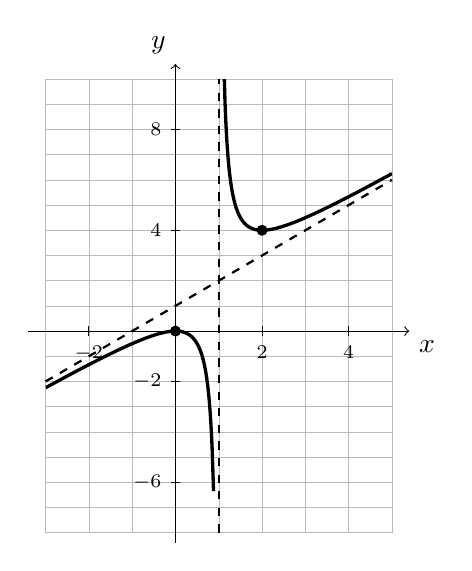
\begin{tikzpicture}[x=0.55cm,y=0.32cm]
  \draw[gray!55,very thin,step=1] (-3,-8) grid (5,10);
  \draw[->] (-3.4,0) -- (5.4,0) node[below right] {$x$};
  \draw[->] (0,-8.4) -- (0,10.6) node[above left] {$y$};
  \foreach \i in {-2,2,4} \draw (\i,0.2) -- (\i,-0.2) node[below,font=\scriptsize] {$\i$};
  \foreach \j in {-6,-2,4,8} \draw (0.1,\j) -- (-0.1,\j) node[left,font=\scriptsize] {$\j$};
  \draw[dashed,thick] (1,-8) -- (1,10);
  \draw[dashed,thick] (-3,-2) -- (5,6);
  \begin{scope}
    \clip (-3,-8) rectangle (5,10);
    \draw[\colorgrafica,very thick,domain=-3:0.88,samples=120,smooth] plot (\x,{(\x*\x)/(\x-1)});
    \draw[\colorgrafica,very thick,domain=1.11:5,samples=120,smooth] plot (\x,{(\x*\x)/(\x-1)});
  \end{scope}
  \fill (0,0) circle (2pt); \fill (2,4) circle (2pt);
\end{tikzpicture}
\end{center}
\end{solucio}

\end{apartats}
